
\begin{figure}
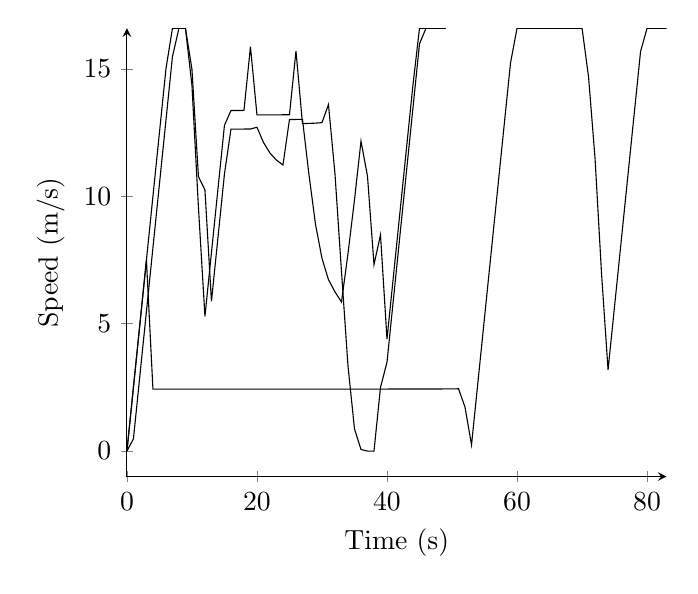
\begin{tikzpicture}
\begin{axis}[
legend style={anchor=west},
axis x line=bottom,
axis y line=left,
ymin=-1,
xlabel=Time (s),
ylabel=Speed (m/s),
]
\addplot[] coordinates {
(0, 0.0)
(1, 2.5)
(2, 5.0)
(3, 7.5)
(4, 2.43354320299)
(5, 2.43354847875)
(6, 2.43355406776)
(7, 2.43355999532)
(8, 2.43356628937)
(9, 2.43357298077)
(10, 2.43358010372)
(11, 2.43358769618)
(12, 2.43359580036)
(13, 2.43360446335)
(14, 2.43361373779)
(15, 2.43362368266)
(16, 2.43363436424)
(17, 2.43364585723)
(18, 2.43365824604)
(19, 2.43367162635)
(20, 2.43368610702)
(21, 2.43370181227)
(22, 2.43371888438)
(23, 2.43373748695)
(24, 2.43375780885)
(25, 2.43378006909)
(26, 2.43380452271)
(27, 2.43383146828)
(28, 2.43386125702)
(29, 2.43389430448)
(30, 2.43393110517)
(31, 2.43397225139)
(32, 2.43401845744)
(33, 2.43407059118)
(34, 2.43412971555)
(35, 2.43419714393)
(36, 2.43427451476)
(37, 2.43436389359)
(38, 2.43446791488)
(39, 2.43458998215)
(40, 2.43473455617)
(41, 2.43490757861)
(42, 2.43511710983)
(43, 2.43537431578)
(44, 2.43569504402)
(45, 2.43610243482)
(46, 2.43663144095)
(47, 2.43733707825)
(48, 2.43831051391)
(49, 2.43971321636)
(50, 2.44185821158)
(51, 2.4454379487)
(52, 1.72380528006)
(53, 0.242716127101)
(54, 2.7427161271)
(55, 5.2427161271)
(56, 7.7427161271)
(57, 10.2427161271)
(58, 12.7427161271)
(59, 15.2427161271)
(60, 16.6)
(61, 16.6)
(62, 16.6)
(63, 16.6)
(64, 16.6)
(65, 16.6)
(66, 16.6)
(67, 16.6)
(68, 16.6)
(69, 16.6)
(70, 16.6)
(71, 14.6887128138)
(72, 11.4859599737)
(73, 6.9586757239)
(74, 3.18820808593)
(75, 5.68820808593)
(76, 8.18820808593)
(77, 10.6882080859)
(78, 13.1882080859)
(79, 15.6882080859)
(80, 16.6)
(81, 16.6)
(82, 16.6)
(83, 16.6)
};
\addplot[] coordinates {
(0, 0.0)
(1, 0.480740698408)
(2, 2.98074069841)
(3, 5.48074069841)
(4, 7.98074069841)
(5, 10.4807406984)
(6, 12.9807406984)
(7, 15.4807406984)
(8, 16.6)
(9, 16.6)
(10, 14.9907174271)
(11, 10.7761896145)
(12, 10.2509967951)
(13, 5.87783377948)
(14, 8.37783377948)
(15, 10.8778337795)
(16, 12.6390809562)
(17, 12.6402439117)
(18, 12.6415985561)
(19, 12.6431894762)
(20, 12.7130642124)
(21, 12.1151356008)
(22, 11.7008757498)
(23, 11.4202517842)
(24, 11.2333810812)
(25, 13.0171406901)
(26, 13.0187101044)
(27, 13.0207931184)
(28, 10.8496875083)
(29, 8.90970435075)
(30, 7.56629932145)
(31, 6.72710792982)
(32, 6.24972828743)
(33, 5.8533203973)
(34, 7.75302007641)
(35, 9.86037266522)
(36, 12.1689611879)
(37, 10.7904686708)
(38, 7.32012741884)
(39, 8.48771074264)
(40, 4.39428851104)
(41, 6.89428851104)
(42, 9.39428851104)
(43, 11.894288511)
(44, 14.394288511)
(45, 16.6)
(46, 16.6)
(47, 16.6)
(48, 16.6)
(49, 16.6)
};
\addplot[] coordinates {
(0, 0.0)
(1, 2.5)
(2, 5.0)
(3, 7.5)
(4, 10.0)
(5, 12.5)
(6, 15.0)
(7, 16.6)
(8, 16.6)
(9, 16.6)
(10, 14.3587818889)
(11, 9.5619605877)
(12, 5.28853800458)
(13, 7.78853800458)
(14, 10.2885380046)
(15, 12.7885380046)
(16, 13.3691000973)
(17, 13.3706158337)
(18, 13.3724130495)
(19, 15.8724130495)
(20, 13.1968409903)
(21, 13.1975986175)
(22, 13.198543142)
(23, 13.1997415733)
(24, 13.201293926)
(25, 13.2033548734)
(26, 15.7033548734)
(27, 12.8554071077)
(28, 12.8626755215)
(29, 12.8741674337)
(30, 12.893955574)
(31, 13.6042698308)
(32, 10.8820653405)
(33, 7.04601460639)
(34, 3.3463941664)
(35, 0.870105815552)
(36, 0.062762087552)
(37, 0.0)
(38, 0.0)
(39, 2.5)
(40, 3.48810918675)
(41, 5.98810918675)
(42, 8.48810918675)
(43, 10.9881091867)
(44, 13.4881091867)
(45, 15.9881091867)
(46, 16.6)
(47, 16.6)
(48, 16.6)
(49, 16.6)
};

\end{axis}
\end{tikzpicture}
\label{tik:speed:100:52}
\caption{100 percent diving with GSC on route $52$}
\end{figure}
